\documentclass[11pt]{article}
\usepackage[T1]{fontenc}
\usepackage[utf8]{inputenc}
\usepackage{lmodern}
\usepackage[margin=1in]{geometry}
\usepackage{amsmath,amssymb,amsthm,mathtools}
\usepackage{enumitem}
\usepackage{microtype}
\usepackage{xcolor}
\usepackage{tikz}
\usetikzlibrary{arrows.meta}
\usepackage[unicode,colorlinks=true,linkcolor=blue!45!black,citecolor=blue!45!black,urlcolor=blue!45!black]{hyperref}
\numberwithin{equation}{section}
\newtheorem{theorem}{Theorem}[section]
\newtheorem{lemma}[theorem]{Lemma}
\newtheorem{proposition}[theorem]{Proposition}
\newtheorem{corollary}[theorem]{Corollary}
\theoremstyle{definition}
\newtheorem{definition}[theorem]{Definition}
\theoremstyle{remark}
\newtheorem{remark}[theorem]{Remark}
\newcommand{\C}{\mathbb C}
\newcommand{\R}{\mathbb R}
\newcommand{\Z}{\mathbb Z}
\newcommand{\Q}{\mathbb Q}
\newcommand{\D}{\mathcal D}
\newcommand{\OO}{\mathcal O}
\newcommand{\Db}{D^{\mathrm b}}
\newcommand{\Knum}{K_{\mathrm{num}}}
\newcommand{\norm}[1]{\left\lVert#1\right\rVert}
\DeclareMathOperator{\Coh}{Coh}
\DeclareMathOperator{\ch}{ch}
\DeclareMathOperator{\rk}{rk}
\DeclareMathOperator{\Hom}{Hom}
\DeclareMathOperator{\Ext}{Ext}
\DeclareMathOperator{\im}{im}
\renewcommand{\Re}{\operatorname{Re}}
\renewcommand{\Im}{\operatorname{Im}}
\setlist{itemsep=3pt,topsep=5pt}
\setlength{\emergencystretch}{1em}
\title{A Gepner stability condition on every smooth quintic threefold}
\author{OpenAI}
\date{September 24, 2026}
\hypersetup{pdftitle={A Gepner stability condition on every smooth quintic threefold},pdfauthor={OpenAI}}
\begin{document}
\maketitle
\begin{abstract}
We prove Toda's normalized quintic Gepner conjecture. On every smooth complex
quintic threefold, we construct a numerical Bridgeland stability condition for
which tensoring by the hyperplane bundle, followed by the spherical twist at
the structure sheaf, increases phase by $2/5$.
\end{abstract}
\section{Introduction}

Stability conditions organize the objects of a derived category by a complex
central charge and a real phase, with finite filtrations into semistable
objects. Their physical antecedent is Douglas's proposal of $\Pi$-stability
for D-branes \cite{Douglas2001}; Bridgeland gave the mathematical framework
used here \cite{Bridgeland2007}. At a Gepner point, one seeks a stability
condition compatible with a distinguished autoequivalence: the functor should
rotate the central charge and translate every semistable phase by a fixed
amount. We construct such a condition for every smooth quintic threefold.

Let $X\subset\mathbb P^4_{\C}$ be a smooth quintic hypersurface, and put
$\D=\Db(\Coh(X))$ and $H=c_1(\OO_X(1))$. The structure sheaf is spherical:
$\Ext^*(\OO_X,\OO_X)=\C\oplus\C[-3]$. Using the spherical twist of
Seidel--Thomas \cite{SeidelThomas2001}, we consider the autoequivalence
\[
 \Phi=T_{\OO_X}\circ(-\otimes\OO_X(1)),\qquad
 T_{\OO_X}(E)=\operatorname{Cone}\bigl(
 R\Hom(\OO_X,E)\otimes\OO_X\longrightarrow E\bigr).
\]
We write $\Knum(X)$ for the Grothendieck group modulo the radical of its Euler
pairing, and $\Knum(X)_{\R}=\Knum(X)\otimes_{\Z}\R$.
A numerical central charge is a homomorphism $Z\colon\Knum(X)\to\C$.

Following Bridgeland \cite{Bridgeland2007}, a slicing $\mathcal P$ is a family
of full additive subcategories $\mathcal P(\varphi)\subset\D$, indexed by
$\varphi\in\R$, with
$\mathcal P(\varphi+1)=\mathcal P(\varphi)[1]$,
vanishing $\Hom(\mathcal P(\varphi_1),\mathcal P(\varphi_2))$ for
$\varphi_1>\varphi_2$, and finite Harder--Narasimhan filtrations by distinguished
triangles with strictly decreasing phases. A nonzero object of
$\mathcal P(\varphi)$ has charge in $\R_{>0}e^{i\pi\varphi}$. Local finiteness
requires the extension categories of sufficiently short phase intervals to be
quasi-abelian of finite length. We use the support property of
Kontsevich--Soibelman \cite[Section~1.2]{KontsevichSoibelman2008}, expressed on
the full numerical group: there exist a norm on $\Knum(X)_{\R}$ and a
constant $C>0$ such that
\[
 \norm{[E]}\le C|Z(E)|
 \quad\text{for every nonzero }E\in\mathcal P(\varphi).
\]
The pair $(Z,\mathcal P)$ is a numerical Bridgeland stability condition when
these charge and slicing requirements hold, with local finiteness.
We will also verify directly that each phase category is closed under direct
summands, using the phase cuts constructed in Lemma~\ref{lem:phase-cuts}.

Toda formulated Gepner-type stability for graded matrix factorizations
\cite[Definition~2.3 and Conjecture~1.2]{Toda2013}, and gave the normalized
quintic formulation in \cite[Conjecture~3.1]{TodaQuintic2013}.
The following theorem positively resolves this quintic conjecture.

\begin{theorem}\label{thm:main}
Every smooth complex quintic threefold admits a numerical Bridgeland stability
condition $\sigma=(Z,\mathcal P)$ with the support property on $\Knum(X)_{\R}$
such that, for every $E\in\D$ and $\varphi\in\R$,
\[
 Z(\Phi E)=e^{2\pi i/5}Z(E),\qquad
 \Phi\bigl(\mathcal P(\varphi)\bigr)=\mathcal P(\varphi+2/5),\qquad
 Z(\OO_x)=-1
\]
for every closed point $x\in X$.
\end{theorem}

The normalization identifies our central charge with Toda's by the uniqueness
of the normalized eigenform proved in Proposition~\ref{prop:central-charge}.

\paragraph{Prior work and the remaining construction.}
The functor relation $\Phi^5\simeq[2]$ and its eigencharge are established
features of the quintic Gepner problem. Orlov's equivalence
\cite[Theorem~2.5]{Orlov2009} and the compatibility with grade shift proved by
Ballard--Favero--Katzarkov \cite[Proposition~5.8 and Remark~5.12]{BallardFaveroKatzarkov2012}
identify the relevant categorical symmetry; Toda recalls this identification
in \cite[Theorem~2.5]{TodaQuintic2013}. A direct computation with
Fourier--Mukai kernels appears in Aspinwall \cite[Section~7.1.4]{Aspinwall2004}.
Section~\ref{sec:numerical} fixes the numerical conventions used in our
construction; Appendix~\ref{app:periodicity} supplies a relative-kernel proof
of the functor relation.

The double-tilt approach to threefold stability was developed by
Bayer--Macr\`i--Toda \cite{BayerMacriToda2014}. For the Gepner charge, Toda
already proposed the first slope tilt at $-1/2$ and the second tilt using
the imaginary part of that charge
\cite[Sections~3.4--3.6 and Conjecture~3.9]{TodaQuintic2013}.
His Remark~3.10 identifies the existence of Harder--Narasimhan filtrations
for this irrational charge as a remaining difficulty.
The existence of numerical Bridgeland stability conditions on every smooth
quintic was established by Li \cite[Theorem~1.3]{Li2019}.
Theorem~\ref{thm:main} adds the specified Gepner symmetry.
Our slope-sheaf input is a consequence
of Xu's stronger Bogomolov--Gieseker inequality
\cite[Theorem~1.3]{Xu2026}, whose hypotheses and precise comparison with the
bound used here are recorded in Lemma~\ref{lem:slope-input}.

\paragraph{Main idea and proof roadmap.}
The central step is to retain two independent perturbations of Toda's second
cut. They give inequalities controlling rank and first Chern character; the
complex charge then controls the other two numerical coordinates. We obtain
this support estimate before defining semistable objects. It makes finite
refinement possible even though the image of the numerical lattice under the
charge need not be discrete.

The proof proceeds through four stages.
\begin{enumerate}
\item In Section~\ref{sec:numerical}, we record periodicity and compute the
unique normalized eigencharge. We also identify the full numerical group
with a rank-four lattice. The resulting coordinate estimate will turn
control of rank, first Chern character, and charge into full support.

\item In Section~\ref{sec:aisles}, we construct a family of bounded aisles
$U_\eta$, where an aisle is the nonpositive part of a bounded
$t$-structure and $\eta=(\eta_0,\eta_1)$ ranges over a fixed open square in
$\R^2$. The construction tilts $\Coh(X)$ twice, beginning at slope
$-1/2$, and varies the rank and first-Chern coefficients of the second cut.
Xu's inequality supplies strict margins for the comparison. The crucial
conclusion of Proposition~\ref{prop:uniform-aisle} is
\[
 \Phi U_{\eta}\subset U_{\theta}.
\]
Both parameters vary independently throughout the same square.

\item In Section~\ref{sec:grid}, periodicity and positivity refine the
translated aisles to a nested grid $V_k$, indexed by integers, with phase
spacing $1/5$ (Proposition~\ref{prop:fine-grid}). The category
$\mathcal S_k=V_k\cap V_{k+1}^\perp$ between consecutive aisles is called
a block; here $\perp$ is right $\Hom$-orthogonality. Its charges lie in a
closed sector of angle $\pi/5$. Each block object belongs to every member
of a suitable perturbed family of hearts. Testing all those perturbations
gives the full support estimate of Proposition~\ref{prop:block-support}.

\item We then refine each block into semistable factors
(Lemma~\ref{lem:block-hn}). Support and a positive projection of the charge
bound the numerical classes of subobjects and the length of any refinement.
The full lattice is discrete, so maximal phases exist and refinement stops.
We merge shared endpoint phases to obtain the slicing, construct its phase
cuts, and prove local finiteness through the exact structure of short phase
intervals (Proposition~\ref{prop:local-finiteness}).
\end{enumerate}

\paragraph{Conventions and prerequisites.}
Our aisle convention is degree $\le0$, so aisles are closed under $[1]$.
For a subcategory $\mathcal C$, the notation
$\mathcal C^\perp$ means its right $\Hom$-orthogonal. Extension closures always
include the zero object and finite iterated extensions. We use standard
coherent-sheaf cohomology, slope Harder--Narasimhan filtrations, derived
truncations, Riemann--Roch, Serre duality, and the hyperplane theorem. The
specific slope inequality is cited as above; the construction of the
stability condition from it is given in full.

\section{Periodicity and the numerical central charge}
\label{sec:numerical}

Throughout, $X\subset\mathbf P^4_{\C}$ is a smooth hypersurface of degree
five, $i\colon X\hookrightarrow\mathbf P^4$ is its inclusion, and
$\D=\Db(\Coh(X))$. Put $H=c_1(\OO_X(1))$, so that $\int_XH^3=5$.
For an object $E\in\D$ we use the normalized characters
\begin{equation}
\label{eq:normalized-characters}
 v(E)=(r,c,d,e)
 =\left(\rk(E),\frac{\int_XH^2\ch_1(E)}5,
                  \frac{\int_XH\ch_2(E)}5,
                  \frac{\int_X\ch_3(E)}5\right).
\end{equation}
In particular, ordinary slope is normalized as $\mu_H(E)=c(E)/r(E)$
for a sheaf of positive rank. We first record the functor relation that
will make the subsequent family of aisles periodic, and then determine
the central charge on the full numerical Grothendieck group.
The periodicity is already visible in Aspinwall's direct kernel calculation
\cite[Section~7.1.4]{Aspinwall2004}. It also follows from Orlov's equivalence
\cite[Theorem~2.5]{Orlov2009} and its compatibility with grade shift
\cite[Proposition~5.8 and Remark~5.12]{BallardFaveroKatzarkov2012},
as recalled in \cite[Theorem~2.5]{TodaQuintic2013}.
Appendix~\ref{app:periodicity} gives a direct proof, keeping track of the
relative kernels and the natural transformations needed for a functor
isomorphism.  Here we record the relation and compute its numerical action.

\begin{lemma}\label{lem:periodicity}
Let $\Phi=T_{\OO_X}\circ(-\otimes\OO_X(1))$. There is a natural
isomorphism of exact functors
\begin{equation}\label{eq:periodicity}
 \Phi^5\simeq[2].
\end{equation}
Consequently $\Phi$ is an autoequivalence, with inverse $\Phi^4[-2]$.
\end{lemma}

To prove the relation, expand the ordered composition as
\[
 \Phi^5\simeq
 T_{\OO_X}\circ T_{\OO_X(1)}\circ\cdots\circ T_{\OO_X(4)}
 \circ(-\otimes\OO_X(5)).
\]
The rightmost functor acts first.  The relative-kernel argument in
Appendix~\ref{app:periodicity} identifies this twist product with
tensoring by $\OO_X(-5)$ followed by $[2]$.

We next identify the entire numerical group and its integral discreteness.
After computing the charge, these coordinates will also show that controlling
rank, first Chern character, and charge suffices to control a numerical class.

\begin{lemma}\label{lem:numerical}
The map $v$ identifies $\Knum(X)_{\R}$ with $\R^4$. Under this
identification, $\Knum(X)$ is a full discrete lattice contained in
\begin{equation}\label{eq:numerical-lattice}
 \Z\times\Z\times\tfrac1{10}\Z\times\tfrac1{30}\Z.
\end{equation}
For $v=(r,c,d,e)$ and $w=(r',c',d',e')$, the Euler form is
\begin{equation}\label{eq:euler-form}
 \chi(v,w)=5\left(re'-cd'+dc'-er'
                   +\frac56(rc'-cr')\right).
\end{equation}
The matrix induced by $\Phi$ is
\begin{equation}\label{eq:numerical-rotation}
 M=
 \begin{pmatrix}
 -4&-20/3&-5&-5\\
 1&1&0&0\\
 1/2&1&1&0\\
 1/6&1/2&1&1
 \end{pmatrix},
 \qquad
 \det(zI-M)=z^4+z^3+z^2+z+1.
\end{equation}
\end{lemma}

\begin{proof}
The Weak Lefschetz Theorem (in the integral form recalled in
\cite[Theorem~3]{Catanese2014}) and Poincar\'e duality give
$H^{2j}(X,\Q)=\Q H^j$ for $0\le j\le3$; the integral version also
gives $H^2(X,\Z)=\Z H$. Thus the even Chern character is precisely
\[
 \ch(E)=r+cH+dH^2+eH^3.
\]
The tangent sequence gives
$c(T_X)=(1+H)^5/(1+5H)$, so that $c_1(T_X)=0$,
$c_2(T_X)=10H^2$, and
\[
 \operatorname{td}(X)=1+\frac56H^2.
\]
Hirzebruch--Riemann--Roch, obtained by taking the proper map to a point in
\cite[Section~7]{BorelSerre1958}, now gives \eqref{eq:euler-form}, and in
particular
\begin{equation}\label{eq:euler-characteristic}
 \chi(E)=5\left(e(E)+\frac56c(E)\right).
\end{equation}
The matrix of the bilinear form~\eqref{eq:euler-form} is
\[
 J=\begin{pmatrix}
 0&25/6&0&5\\
 -25/6&0&-5&0\\
 0&5&0&0\\
 -5&0&0&0
 \end{pmatrix},
 \qquad\det J=625.
\]
Moreover the four vectors
\[
 v(\OO_X(k))=(1,k,k^2/2,k^3/6),\qquad 0\le k\le3,
\]
span $\Q^4$: their row matrix has determinant one. It follows that
the kernel of $v$ on $K_0(X)$ is exactly the radical of the Euler
pairing. Indeed one implication follows from Riemann--Roch, and the
other follows by testing against these four spanning vectors and using
the nondegeneracy of $J$. Hence $v$ identifies the numerical group with
its image, which spans $\Q^4$.

For any class of $K_0(X)$, integrality of Chern classes and
\[
 \ch_2=\frac{c_1^2-2c_2}{2},\qquad
 \ch_3=\frac{c_1^3-3c_1c_2+3c_3}{6}
\]
give $d\in\tfrac1{10}\Z$ and $e\in\tfrac1{30}\Z$; integral Weak
Lefschetz gives $c\in\Z$. The image is therefore a subgroup of the
discrete lattice in \eqref{eq:numerical-lattice}. Since it contains the
four spanning line-bundle classes, it is itself a full lattice.
In particular its real span is the full space $\R^4$.

Tensoring by $\OO_X(1)$ sends
\[
 (r,c,d,e)\longmapsto
 \left(r,c+r,d+c+\frac r2,e+d+\frac c2+\frac r6\right).
\]
The twist $T_{\OO_X}$ then subtracts $\chi(E(1))$ from the rank and leaves
the other three coordinates unchanged. Formula~\eqref{eq:euler-characteristic}
therefore gives $M$ as displayed. Expanding $\det(zI-M)$ gives
\eqref{eq:numerical-rotation}; in particular its four eigenvalues are
the nonidentity fifth roots of unity, each with multiplicity one.
\end{proof}

We denote by $\Phi_*$ the induced automorphism of $\Knum(X)$ and its
real-linear extension to $\Knum(X)_{\R}$; both are represented by $M$ in
these coordinates.

Put
\begin{equation}\label{eq:charge-constants}
 \lambda=\exp(2\pi i/5),\qquad
 t_0=\frac12\cot(\pi/5)>0,\qquad
 u=\frac45\sin^2(\pi/5)=\frac{5-\sqrt5}{10}.
\end{equation}

\begin{proposition}\label{prop:central-charge}
There is a unique numerical homomorphism $Z\colon\Knum(X)\to\C$
such that $Z\circ\Phi=\lambda Z$ and $Z(\OO_x)=-1$ for closed points
$x\in X$. It is
\begin{equation}\label{eq:central-charge}
 \frac{Z(r,c,d,e)}5
  =\frac{\lambda-1}{5}r
   +\left(t_0^2-\frac56+\frac{i t_0}{2}\right)c
   +\left(-\frac12+i t_0\right)d-e.
\end{equation}
In particular,
\begin{equation}\label{eq:imaginary-charge}
 \frac{\Im Z(r,c,d,e)}{5t_0}=d+\frac12c+ur.
\end{equation}
For any fixed norm on $\Knum(X)_{\R}$, there is a constant $C_0>0$
such that every real numerical class $v=(r,c,d,e)$ satisfies
\begin{equation}\label{eq:numerical-norm-control}
 \norm{v}\le C_0\bigl(|r|+|c|+|Z(v)|\bigr).
\end{equation}
\end{proposition}

\begin{proof}
A closed point has $v(\OO_x)=(0,0,0,1/5)$, so the normalization fixes
the coefficient of $e$ in $Z/5$ to be $-1$.
Write $Z/5=Ar+Bc+Cd-e$. Reading the $e$, $d$, and $c$ columns of
$ZM=\lambda Z$, in that order, gives
\[
 A=\frac{\lambda-1}{5},\qquad
 C=-\frac{\lambda}{\lambda-1},\qquad
 B=-\frac43+\frac{C-1/2}{\lambda-1}.
\]
The identity
\[
 \frac1{\lambda-1}=-\frac12-i t_0
\]
then gives $C=-1/2+i t_0$ and
$B=t_0^2-5/6+i t_0/2$. Substitution in the remaining, rank-column
equation reduces it to
$1+\lambda+\lambda^2+\lambda^3+\lambda^4=0$.
This proves both the eigenvalue identity and uniqueness with the stated
normalization. Taking imaginary parts and using
\[
 \frac{\sin(2\pi/5)}{5t_0}
       =\frac45\sin^2(\pi/5)=u
\]
proves \eqref{eq:imaginary-charge}.

Finally, the real coefficient matrix of $(d,e)$ in
$(\Re Z,\Im Z)$ is
\[
 \begin{pmatrix}-5/2&-5\\5t_0&0\end{pmatrix},
 \qquad \det=25t_0\ne0.
\]
Thus $v\mapsto(r,c,\Re Z(v),\Im Z(v))$ is an isomorphism of real
vector spaces. Boundedness of its inverse in finite dimension proves
\eqref{eq:numerical-norm-control}.
\end{proof}

\section{A uniform family of double-tilt aisles}
\label{sec:aisles}

Our goal is to construct bounded aisles $U_\eta$ for which
$\Phi U_\eta\subset U_\theta$ holds uniformly with independent parameters.
We begin with Toda's proposed two tilts for the quintic Gepner charge
\cite[Sections~3.4--3.6]{TodaQuintic2013}, and vary the second cut in two
numerical directions. The slope estimate below supplies the strict margins
that make the comparison survive these variations.
The two first-tilt slopes $-1/2$ and $1/2$ reflect the order of the factors
in $\Phi$: tensoring by $\OO_X(1)$ moves the first cut from $-1/2$ to
$1/2$, and the spherical twist will take the resulting aisle into one
constructed at $-1/2$.

We first isolate the geometric input.  Slope always means
$\mu(F)=c(F)/r(F)$ for a torsion-free sheaf of positive rank.  We use
ordinary slope Harder--Narasimhan filtrations, writing $\mu^+(F)$ and
$\mu^-(F)$ for their largest and smallest slopes.  For an arbitrary
sheaf, its torsion subsheaf is removed before these slopes are taken.

\begin{lemma}[Slope input]\label{lem:slope-input}
Put
\[
 f(x)=\max\left\{-\frac{3x}{25},\ \frac{x}{2}-\frac7{25},\
                    \frac{28x}{25}-\frac{31}{50}\right\}
                    \qquad(0\leq x\leq1).
\]
Every torsion-free slope-semistable sheaf $F$ on $X$ with
$|\mu(F)|\leq1$ satisfies
\begin{equation}\label{eq:slope-envelope}
                 \frac{d(F)}{r(F)}\leq f(|\mu(F)|).
\end{equation}
The estimate extends under integral twists by
$(x,y)\mapsto(x+n,y+nx+n^2/2)$.  In particular,
$f(x)\leq0$ for $0\leq x\leq1/2$, and $f(1/2)=-3/100$.
\end{lemma}

\begin{proof}
We use Xu's Theorem~1.3 \cite{Xu2026}.  Its hypotheses are precisely a
smooth complex quintic threefold with its hyperplane polarization and a
torsion-free slope-semistable sheaf of slope in $[-1,1]$; its coordinates
$\mu_H$ and $\xi_H$ are our $c/r$ and $d/r$.  On $[0,1/2]$ its upper
bound $g$ is
\[
g(x)=
\begin{cases}
-x/2,&0\leq x\leq1/4,\\
x/2-1/4,&1/4\leq x\leq5/13,\\
-3x/20,&5/13\leq x\leq6/13,\\
x/2-3/10,&6/13\leq x\leq1/2.
\end{cases}
\]
The first and third lines are at most $-3x/25$; the second is also at
most $-3x/25$ because $5/13<25/62$; and the last is at most
$x/2-7/25$.  Thus $g\leq f$ on this half interval.  The full upper
bound $g$ in Xu's theorem and the maximum $f$ both satisfy
\[
 h(1-x)=h(x)+\frac12-x.
\]
For $f$, this reflection exchanges the first and third affine pieces
and fixes the second.  This proves the comparison on $[0,1]$, and the
theorem uses $|\mu|$ on the negative strip.

For completeness, the symmetry is also compatible with the sheaf
operations used here.  Twisting by $\OO_X(n)$ has the displayed effect
on $(x,y)$ and preserves slope semistability.  If $F$ is not reflexive,
passing to $F^{**}$ preserves slope semistability and $r,c$, and only
increases $d$.  For a reflexive sheaf on a smooth threefold the higher
sheaf Ext terms of its derived dual are supported in dimension zero,
so its ordinary dual has characters $(r,-c,d)$ through degree two and
is slope-semistable.  The operations of dualizing and twisting by
$\OO_X(1)$ therefore give $(x,y)\mapsto(1-x,y+1/2-x)$ without changing
the validity of an upper bound.  Finally the three defining lines are
nonpositive on $[0,1/2]$, and their maximum at $1/2$ is $-3/100$.
\end{proof}

We use aisles in the convention $\D^{\leq0}$: they are closed under
$[1]$, and the heart of an aisle $V$ is $V\cap(V[1])^\perp$, where
$\perp$ denotes right Hom orthogonality.  Recall explicitly the tilt
construction of Happel--Reiten--Smal\o\ \cite{HappelReitenSmalo1996}.
A torsion pair $(\mathcal T,\mathcal F)$ in the heart of
a bounded aisle $V$ gives the aisle
\begin{equation}\label{eq:aisle-tilt}
 V^\sharp=\{E\in V:H^0_V(E)\in\mathcal T\},\qquad
 \mathcal H^\sharp=\langle\mathcal F[1],\mathcal T\rangle,
 \qquad V[1]\subset V^\sharp\subset V.
\end{equation}
Here and below angle brackets denote extension closure.  To construct
the new truncation triangle, first truncate at zero for $V$, then take
the inverse image of the torsion subobject of its zeroth cohomology.
The remaining triangle has terms from $\mathcal F$ and the old positive
degrees.  The old orthogonality and
$\Hom(\mathcal T,\mathcal F)=0$ give the required new orthogonality.
Shift closure and the two inclusions prove that this is a bounded
$t$-structure.  The same truncations show conversely that an aisle
between $V[1]$ and $V$ gives a torsion pair in the heart of $V$.

For $b\in\{-1/2,1/2\}$, let $\mathcal C_{\leq b}$ consist of zero
and the torsion-free sheaves with $\mu^+\leq b$, and let
$\mathcal C_{>b}$ consist of sheaves whose torsion-free quotient has
$\mu^->b$, together with all torsion sheaves.  Ordinary slope
filtrations give the torsion pair
$(\mathcal C_{>b},\mathcal C_{\leq b})$ in $\Coh(X)$.  Define the
first tilted heart and its aisle by
\[
 \mathcal B_b=\langle\mathcal C_{\leq b}[1],\mathcal C_{>b}\rangle,
 \qquad W_b=\D^{\leq0}_{\mathcal B_b},
 \qquad p_b=c-br.
\]
On $\mathcal B_b$, $p_b$ takes values in $\frac12\Z_{\geq0}$, by
Lemma~\ref{lem:numerical}.  For $E\in\mathcal B_b$, the equality
$p_b(E)=0$ holds exactly when $H^{-1}(E)$ is slope-semistable of slope
$b$ (or zero), and $H^0(E)$ has dimension at most one.  This follows
by applying $p_b$ to the slope factors of the two cohomology sheaves:
each contribution is nonnegative, and a nonzero divisorial torsion
sheaf has positive $c$.

\begin{lemma}\label{lem:first-tilt-noetherian}
The abelian categories $\mathcal B_{-1/2}$ and $\mathcal B_{1/2}$ are
noetherian.
\end{lemma}

\begin{proof}
We give the rational first-tilt argument; compare
\cite[proof of Lemma~3.2.4]{BayerMacriToda2014}.
Consider epimorphisms $E_0\twoheadrightarrow E_1\twoheadrightarrow
E_2\twoheadrightarrow\cdots$ in $\mathcal B_b$, with kernels $K_i$
for the individual arrows.  The nonnegative discrete numbers
$p_b(E_i)$ eventually stabilize, so $p_b(K_i)=0$.  The ordinary
cohomology sheaves $H^0(E_i)$ form a sequence of epimorphisms and
eventually stabilize, since $\Coh(X)$ is noetherian.  The preceding
description of $K_i$ gives $r(K_i)\leq0$, hence the integers $r(E_i)$
are nondecreasing.  They are bounded above by the now fixed rank of
$H^0(E_i)$, so eventually $r(K_i)=0$.  Each remaining $K_i$ is then an
ordinary sheaf of dimension at most one.

The cohomology sequence now reads
\[
 0\longrightarrow H^{-1}(E_i)\longrightarrow H^{-1}(E_{i+1})
   \longrightarrow K_i\longrightarrow0.
\]
These torsion-free sheaves agree in codimension one.  Their injections
extend to isomorphisms of their reflexive hulls, so they form an
increasing chain of coherent subsheaves of a fixed reflexive sheaf.
That chain stabilizes, forcing $K_i=0$.  Thus every such sequence of
epimorphisms stabilizes, as required.
\end{proof}

The first tilted hearts are now available. We define the second cut and choose
constants for three uses: negativity at the slope boundary, exclusion of a
small neighboring slope strip, and a strict comparison between the two cuts.
At zero perturbation and $b=-1/2$, the cut is the imaginary part of the
normalized Gepner charge, as in Toda's candidate heart
\cite[Section~3.6]{TodaQuintic2013}. Fix
\begin{equation}\label{eq:aisle-parameters}
 \begin{gathered}
 \delta=10^{-5},\qquad s_0=\frac{553}{1000},\qquad
 B_\delta=\{\eta=(\eta_0,\eta_1)\in\R^2:|\eta_j|<\delta\},\\
 N_b^\eta=d-bc+ur+\eta_1c+\eta_0r.
 \end{gathered}
\end{equation}
The following exact margins will be useful:
\begin{align}
 m_b&=\frac7{25}-u-\frac32\delta>0,\label{eq:boundary-margin}\\
 m_s&=\frac{13857}{50000}-u-(1+s_0)\delta>0,
                                                    \label{eq:strip-margin}\\
 m_c&=\frac12-\frac{u}{s_0}-3\delta>0.\label{eq:comparison-margin}
\end{align}
For example, $\sqrt5>223606/100000$ implies
$u<138197/500000$, and gives respectively the positive lower bounds
$3591/10^6$, $73047/10^8$, and $8941/55300000$ for these three
expressions.  On a slope-semistable sheaf $F$ of slope $b$,
Lemma~\ref{lem:slope-input} gives
\begin{equation}\label{eq:boundary-negative}
 \frac{N_b^\eta(F)}{r(F)}
 \leq -\frac3{100}-\frac14+u+\frac32\delta=-m_b<0.
\end{equation}
Consequently $N_b^\eta\geq0$ on the $p_b=0$ objects of $\mathcal B_b$;
equality holds precisely for zero-dimensional sheaves, including zero.
Indeed their degree-minus-one part contributes strictly positively
unless it vanishes, while a sheaf of dimension at most one has
$N_b^\eta=d\geq0$, with equality exactly in dimension zero.

Call a nonzero object of $\mathcal B_b$ \emph{high} if $p_b=0$ or
$N_b^\eta>0$, and \emph{low} otherwise.  Thus low means $p_b>0$ and
$N_b^\eta\leq0$.  Set
\[
\begin{split}
 \mathcal T_b^\eta&=\{E:\text{every nonzero quotient of $E$ in
                                  $\mathcal B_b$ is high}\},\\
 \mathcal F_b^\eta&=\{E:\text{every nonzero subobject of $E$ in
                                  $\mathcal B_b$ is low}\}.
\end{split}
\]

\begin{lemma}[The second tilt]\label{lem:second-tilt}
For every $b=\pm1/2$ and $\eta\in B_\delta$, the pair
$(\mathcal T_b^\eta,\mathcal F_b^\eta)$ is a torsion pair.  Its tilt
has bounded heart and aisle
\[
 \mathcal A_b^\eta=\langle\mathcal F_b^\eta[1],\mathcal T_b^\eta\rangle,
 \qquad \mathcal U_b^\eta
   =\{E\in W_b:H^0_{\mathcal B_b}(E)\in\mathcal T_b^\eta\}.
\]
On $\mathcal A_b^\eta$ one has $N_b^\eta\geq0$, and no nonzero object
of this heart has zero numerical class.
\end{lemma}

\begin{proof}
High objects are closed under extensions: if one end term has positive
$N_b^\eta$, so does the extension, and otherwise both have $p_b=0$.
It follows, by taking the induced filtration on a quotient, that
$\mathcal T_b^\eta$ is closed under quotients and extensions.

If an object has a high subobject, choose such a nonzero subobject $A$
with $p_b(A)$ minimal.  When $p_b(A)=0$, all its quotients have
$p_b=0$.  Otherwise $N_b^\eta(A)>0$, and a low quotient $Q$ would
have $p_b(Q)>0$ and $N_b^\eta(Q)\leq0$.  Its kernel would then be a
high subobject with strictly smaller $p_b$, a contradiction.  Thus
$A\in\mathcal T_b^\eta$ in either case.

By Lemma~\ref{lem:first-tilt-noetherian}, every object has a maximal
$\mathcal T_b^\eta$ subobject; sums of such subobjects again belong to
$\mathcal T_b^\eta$, so maximality has its usual torsion meaning.  The
quotient has no high subobject, since such a subobject would contain
a nonzero member of $\mathcal T_b^\eta$ by the preceding paragraph,
and its inverse image would enlarge the maximal torsion subobject.
The quotient therefore lies in $\mathcal F_b^\eta$.  Finally a
nonzero image of a map from $\mathcal T_b^\eta$ to
$\mathcal F_b^\eta$ would be both high and low.  This proves the
torsion pair, and \eqref{eq:aisle-tilt} gives boundedness.

Write an object of the new heart as an extension of $T$ by $F[1]$,
where $T\in\mathcal T_b^\eta$ and $F\in\mathcal F_b^\eta$.  Then
$N_b^\eta(T)\geq0$ and $N_b^\eta(F)\leq0$, proving nonnegativity.
If $N_b^\eta(E)=0$, both terms have $N_b^\eta=0$.  Since $T$ itself
is high when nonzero, this forces $p_b(T)=0$, hence $T$ is
zero-dimensional.  If $F\ne0$, then $p_b(F)>0$ and
$p_b(E)=-p_b(F)<0$.  Thus $[E]=0$ would force $F=0$; it would then
force $T=0$, since $e(T)=\operatorname{length}(T)/5$.  This proves
the last assertion.
\end{proof}

We next compare the two slope cuts with independent parameters.
Subscripts $-$ and $+$ mean $b=-1/2$ and $b=1/2$, respectively.

\begin{lemma}\label{lem:compare-slope-cuts}
For every $\alpha,\theta\in B_\delta$,
\[
                       \mathcal U_+^\alpha\subset\mathcal U_-^\theta.
\]
\end{lemma}

\begin{proof}
Let $\mathcal M$ be the ordinary torsion-free sheaves all of whose
slopes lie in $(-1/2,1/2]$, and let
\[
 \mathcal L=\langle\mathcal C_{\leq-1/2}[1],\mathcal C_{>1/2}\rangle
             =\mathcal B_-\cap\mathcal B_+.
\]
To see the torsion pair $(\mathcal L,\mathcal M)$ in $\mathcal B_-$,
take $E\in\mathcal B_-$ and let $M_E$ be the quotient of $H^0(E)$
obtained by removing its torsion and its slope factors above $1/2$.
Then $M_E\in\mathcal M$.  The kernel of $E\to M_E$ in
$\mathcal B_-$ has degree-minus-one cohomology $H^{-1}(E)$ and
degree-zero cohomology in $\mathcal C_{>1/2}$, so it lies in
$\mathcal L$.  The slope vanishing and the ordinary cohomological
degrees give $\Hom(\mathcal L,\mathcal M)=0$.
Tilting this torsion pair gives
$\mathcal B_+=\langle\mathcal M[1],\mathcal L\rangle$; in
$\mathcal B_+$ the corresponding torsion pair is
$(\mathcal M[1],\mathcal L)$.  In particular
$W_-[1]\subset W_+\subset W_-$, and
$W_+[1]\subset W_-[1]\subset\mathcal U_-^\theta$.
It suffices to prove
\begin{equation}\label{eq:comparison-hom}
               \Hom(\mathcal T_+^\alpha,\mathcal F_-^\theta)=0.
\end{equation}
Indeed an object $E\in W_-$ has maps to a member of
$\mathcal F_-^\theta$ exactly through $H^0_{\mathcal B_-}(E)$;
vanishing of all such maps puts this cohomology object in
$\mathcal T_-^\theta$.  Equation~\eqref{eq:comparison-hom} therefore
puts $\mathcal T_+^\alpha$ in $\mathcal U_-^\theta$, and the preceding
inclusion handles the negative $\mathcal B_+$ degrees.

Suppose there is a nonzero map $E\to G$ with
$E\in\mathcal T_+^\alpha$ and $G\in\mathcal F_-^\theta$.
Its source decomposes in $\mathcal B_+$ as
$0\to M_E[1]\to E\to E_0\to0$, with $E_0\in\mathcal L$.
Because $\Hom(\mathcal M[1],\mathcal B_-)=0$, the map factors through
$E_0$, which is still in $\mathcal T_+^\alpha$.  The
$(\mathcal L,\mathcal M)$ decomposition of $G$ in $\mathcal B_-$
then factors it through a subobject $G_0\in\mathcal L$ of $G$, since
$\Hom(\mathcal L,\mathcal M)=0$.

Take the kernel $K$ and the nonzero image $Q$ of $E_0\to G_0$ in
$\mathcal B_-$.  Let $K_{\mathcal L}$ be the $\mathcal L$ torsion
part of $K$, and put $U'=E_0/K_{\mathcal L}$ in $\mathcal B_-$.
The quotient closure of $\mathcal L$ gives $Q,U'\in\mathcal L$.
All three terms of
$K_{\mathcal L}\to E_0\to U'$ belong to both hearts, so its triangle
is short exact in $\mathcal B_+$ as well.  Thus $U'$ remains a
quotient of $E$ in $\mathcal B_+$, and we have
\begin{equation}\label{eq:common-heart-sequence}
 0\longrightarrow S\longrightarrow U'\longrightarrow Q\longrightarrow0
 \quad\text{in }\mathcal B_-,\qquad
 S=K/K_{\mathcal L}\in\mathcal M,
 \quad U'\in\mathcal T_+^\alpha,
 \quad 0\ne Q\in\mathcal F_-^\theta.
\end{equation}
We use the sequence~\eqref{eq:common-heart-sequence} only as a short exact
sequence in $\mathcal B_-$; its term $S$
need not belong to $\mathcal B_+$.

We now use the slope envelope to exclude factors close to the two slope
boundaries. The resulting rank bounds will contradict the opposite signs of
the two cut forms on $U'$ and $Q$.

Directly from the three affine functions defining $f$,
\begin{equation}\label{eq:strip-test}
 \max_{1/2\leq s\leq s_0}\bigl(f(s)-s/2+u\bigr)
                 =u-\frac{13857}{50000}.
\end{equation}
The perturbation error on a slope $\pm s$ is at most
$(1+s_0)\delta$, so \eqref{eq:strip-margin} makes the relevant
sheaf value of $N_-$ on $[-s_0,-1/2]$, or of $N_+$ on
$[1/2,s_0]$, strictly negative.

Write $A=H^{-1}(Q)$.  If $A\ne0$, its top slope factor $A_1$
is a saturated subsheaf and $A/A_1\in\mathcal C_{\leq-1/2}$.
Consequently $A_1[1]$ is a subobject of $A[1]$, and then of $Q$, in
$\mathcal B_-$.  If $\mu(A_1)\in[-s_0,-1/2]$, the preceding
negative sheaf value makes $A_1[1]$ high, contradicting
$Q\in\mathcal F_-^\theta$.  Thus $\mu^+(A)<-s_0$.

For $U'$, put $A'=H^{-1}(U')$ and $D'=H^0(U')$.
If $D'$ has positive rank, remove its ordinary torsion subsheaf and
take its bottom positive-rank slope quotient $G'$.  The kernel of
$D'\to G'$ consists of that torsion and the other slope factors,
all of slope $>1/2$; this sequence is therefore exact in
$\mathcal B_+$.  The ordinary cohomology sequence also makes $D'$
a $\mathcal B_+$ quotient of $U'$, so $G'$ is such a quotient.
A slope $\mu(G')\in(1/2,s_0]$ would give
$p_+(G')>0$, $N_+^\alpha(G')<0$, contradicting
$U'\in\mathcal T_+^\alpha$.  Every positive-rank slope of $D'$
therefore exceeds $s_0$.

For any $L\in\mathcal L$, its two ordinary cohomology sheaves give
\begin{equation}\label{eq:overlap-rank-bound}
 c(L)\geq\frac12\bigl(r(H^{-1}(L))+r(H^0(L))\bigr)
                                     \geq\frac12|r(L)|.
\end{equation}
Divisorial torsion contributes nonnegative $c$, and torsion in lower
dimension contributes zero.  The stronger slope conclusions just
proved similarly give
\begin{equation}\label{eq:two-slope-tests}
          c(Q)\geq-s_0r(Q),\qquad c(U')\geq s_0r(U').
\end{equation}
More explicitly, with $D=H^0(Q)$ the estimates are
\[
 \begin{split}
 c(Q)&\geq s_0r(A)+\tfrac12r(D)\geq-s_0r(Q),\\
 c(U')&\geq\tfrac12r(A')+s_0r(D')\geq s_0r(U').
 \end{split}
\]
They include torsion cohomology sheaves: their ranks are zero and
their contributions to $c$ are nonnegative.  Also $d(S)\leq0$, by applying
Lemma~\ref{lem:slope-input} to the ordinary slope factors of $S$.

Set $C=c(Q)+c(U')$.  By \eqref{eq:overlap-rank-bound}, $C\geq0$.
If $C=0$, then $c(Q)=r(Q)=0$, so $p_-(Q)=0$, impossible for a
nonzero member of $\mathcal F_-^\theta$.  Hence $C>0$; and
\eqref{eq:two-slope-tests} together with
\eqref{eq:common-heart-sequence} gives $C\geq s_0r(S)$.
By additivity,
\begin{align*}
 N_-^\theta(Q)-N_+^\alpha(U')
 &=\frac12 C-u r(S)-d(S)
       +\theta_1c(Q)+\theta_0r(Q)-\alpha_1c(U')-\alpha_0r(U')\\
 &\geq \left(\frac12-\frac{u}{s_0}-3\delta\right)C-d(S)>0.
\end{align*}
Here the absolute value of the last four terms is at most $3\delta C$
by \eqref{eq:overlap-rank-bound}; this applies even when a derived
rank is negative.  The strict sign is \eqref{eq:comparison-margin}.
But $N_-^\theta(Q)\leq0\leq N_+^\alpha(U')$, a contradiction.
This proves \eqref{eq:comparison-hom} and the aisle inclusion.
\end{proof}

\begin{lemma}\label{lem:twist-aisle}
For all $\alpha,\theta\in B_\delta$,
\[
 \OO_X\in\mathcal A_-^\theta,\qquad
 \OO_X[2]\in\mathcal A_+^\alpha,\qquad
 T_{\OO_X}(\mathcal U_+^\alpha)\subset\mathcal U_-^\theta.
\]
\end{lemma}

\begin{proof}
The object $\OO_X\in\mathcal B_-$ has the smallest positive value
$p_-=1/2$ and $N_-^\theta=u+\theta_0>0$.
It has no nonzero subobject of $p_-=0$: a $p_-=0$ object is an
extension of a sheaf of dimension at most one by $F[1]$ of slope
$-1/2$, and both have zero Hom to $\OO_X$.
Any nonzero low quotient of $\OO_X$ would have $p_-=1/2$, leaving
a kernel of $p_-=0$; that kernel must vanish, contradicting that
$\OO_X$ is high.  Hence $\OO_X\in\mathcal T_-^\theta$.

Similarly $\OO_X[1]\in\mathcal B_+$ has $p_+=1/2$ and
$N_+^\alpha=-u-\alpha_0<0$.  A $p_+=0$ object has no map to it:
for its slope-$1/2$ part this is
$\Hom(F[1],\OO_X[1])=\Hom(F,\OO_X)=0$, and for its
dimension-at-most-one part $T$ it follows from
\[
 \Ext^1(T,\OO_X)=H^2(X,T)^*=0.
\]
Here we use Serre duality and $K_X\simeq\OO_X$.  Every nonzero
subobject $A$ of $\OO_X[1]$ therefore has $p_+(A)=1/2$, and its
quotient $Q$ has $p_+(Q)=0$.  Hence
$N_+^\alpha(A)=N_+^\alpha(\OO_X[1])-N_+^\alpha(Q)<0$.
This proves $\OO_X[1]\in\mathcal F_+^\alpha$, and thus
$\OO_X[2]\in\mathcal A_+^\alpha$.

For $B\in\mathcal U_+^\alpha$ and $j\geq2$, Serre duality and
the heart orthogonality give
\[
 \Ext^j(\OO_X,B)
       =\Hom(B[j-1],\OO_X[2])^*=0,
\]
since $B[j-1]\in\mathcal U_+^\alpha[1]$.
Lemma~\ref{lem:compare-slope-cuts} puts $B$ in
$\mathcal U_-^\theta$.  In the twist triangle
\[
 B\longrightarrow T_{\OO_X}(B)\longrightarrow
          \operatorname{RHom}(\OO_X,B)\otimes\OO_X[1]\longrightarrow B[1],
\]
the third term is a finite direct sum of copies of
$\OO_X[1-j]$ with $j\leq1$, because bounded complexes of
finite-dimensional vector spaces split into their cohomology.
All these terms lie in $\mathcal U_-^\theta$.  Extension closure
therefore gives the claimed twist inclusion.
\end{proof}

\begin{proposition}[Uniform independent-parameter inclusion]
\label{prop:uniform-aisle}
There is a fixed open square
\begin{equation}\label{eq:fixed-omega}
 \Omega=\{\eta=(\eta_0,\eta_1):|\eta_0|,|\eta_1|<5\cdot10^{-6}\}
\end{equation}
and bounded aisles $U_\eta=\mathcal U_-^\eta$, with hearts
$\mathcal A_\eta=U_\eta\cap(U_\eta[1])^\perp$, such that
\begin{equation}\label{eq:uniform-aisle}
                    \Phi U_\eta\subset U_\theta
                    \qquad(\eta,\theta\in\Omega).
\end{equation}
Moreover
\begin{equation}\label{eq:perturbed-positive-form}
 N_\eta=d+\frac12c+ur+\eta_1c+\eta_0r\geq0
                    \quad\text{on }\mathcal A_\eta,
 \qquad N_0=\frac{\Im Z}{5t_0},
\end{equation}
and no nonzero object of any $\mathcal A_\eta$ has zero numerical
class.  The two parameters in \eqref{eq:uniform-aisle} vary
independently throughout this same square.
\end{proposition}

\begin{proof}
Tensoring by $\OO_X(1)$ takes $\mathcal B_-$ to $\mathcal B_+$
and preserves the $p$ test.  Its effect on the other test is
\[
 N_+^\alpha(E(1))=N_-^\eta(E)
 \quad\text{when}\quad
             \alpha_1=\eta_1,\qquad\alpha_0=\eta_0-\eta_1.
\]
Thus it takes the second torsion pair and aisle to those with this
parameter $\alpha$.  If $\eta\in\Omega$, then $\alpha\in B_\delta$;
also $\theta\in\Omega$ implies $\theta\in B_\delta$.
Lemma~\ref{lem:twist-aisle} now gives
\[
 \Phi U_\eta=T_{\OO_X}\bigl(\mathcal U_+^\alpha\bigr)
                                      \subset U_\theta.
\]
The remaining assertions are Lemma~\ref{lem:second-tilt} and
\eqref{eq:imaginary-charge}.

The parameter shear was used once, in proving this inclusion for
the original family.  In particular, applying any power $\Phi^i$
to \eqref{eq:uniform-aisle} gives
$\Phi^{i+1}U_\eta\subset\Phi^iU_\theta$ with the same
$\eta,\theta\in\Omega$; it performs no further shear and requires
no further shrinkage.  Negative powers are allowed by
Lemma~\ref{lem:periodicity}.
\end{proof}

\section{From uniform aisle inclusions to a slicing}
\label{sec:grid}

We now use the bounded aisles $U_\eta$ and their hearts
$\mathcal A_\eta$ constructed above.  The parameter $\eta=(\eta_0,\eta_1)$
ranges over the fixed open square $\Omega$ of
Proposition~\ref{prop:uniform-aisle}, and $0\in\Omega$.  The inputs to this
section are
\begin{equation}\label{eq:grid-inputs}
 \begin{gathered}
 \Phi U_\eta\subset U_\theta
 \quad(\eta,\theta\in\Omega),\\
 N_\eta=d+\tfrac12c+ur+\eta_1c+\eta_0r\ge0
 \quad\text{on }\mathcal A_\eta,
 \end{gathered}
\end{equation}
the absence of nonzero objects of zero numerical class in these hearts,
and Lemma~\ref{lem:periodicity}, Lemma~\ref{lem:numerical}, and
Proposition~\ref{prop:central-charge}.  In particular, throughout this
section $\Phi$ is an autoequivalence, $\Phi^5\simeq[2]$, and
$Z\Phi=e^{2\pi i/5}Z$.  All extension closures below mean finite extension
closures, contain zero, and are strictly full subcategories of $\D$.
For a subcategory $\mathcal C$, write
$\mathcal C^\perp=\{E:\Hom(C,E)=0\text{ for all }C\in\mathcal C\}$;
the left orthogonal ${}^\perp\mathcal C$ is defined similarly.

The decisive use of the perturbations is twofold.  Simultaneous positivity
in fixed middle hearts improves the coarse nesting to a grid with spacing
$1/5$.  Positivity in every perturbed preceding heart then bounds the full
numerical class of each grid block by its charge.

\subsection{The finer grid}

Put $D_i^\eta=\Phi^iU_\eta$ for $i\in\Z$.  The hypotheses give
\begin{equation}\label{eq:coarse-grid}
 D_{i+1}^\eta\subset D_i^\theta\quad
 (i\in\Z,\ \eta,\theta\in\Omega),\qquad
 D_{i+5}^\eta=D_i^\eta[2].
\end{equation}
All successive inclusions allow independent parameter choices.
The charge rotation suggests how to insert a fifth-step between these
coarse cuts: $\Phi^3[-1]$ multiplies $Z$ by $e^{i\pi/5}$.
For its translates to give nested aisles, we need
$\Phi^3U_\alpha[-1]\subset U_\beta$, or equivalently
$D_3^\alpha\subset D_0^\beta[1]$.  The next proposition proves this
inclusion before any slicing or semistable phase is defined.

\begin{proposition}[Uniform refinement of the grid]\label{prop:fine-grid}
There is an open square $\Omega_1$ about zero, contained in $\Omega$, such
that
\begin{equation}\label{eq:single-shift-inclusion}
 D_3^\alpha\subset D_0^\beta[1]
 \qquad(\alpha,\beta\in\Omega_1).
\end{equation}
For $k\in\Z$ and $\eta\in\Omega_1$, define
\begin{equation}\label{eq:fifths-aisles}
 V_k^\eta=\Phi^mU_\eta[j],\qquad k=2m+5j.
\end{equation}
This is independent of the integers $m,j$ chosen, and these bounded aisles
satisfy
\begin{equation}\label{eq:fifths-nesting}
 \begin{gathered}
 V_{k+1}^\alpha\subset V_k^\beta,\qquad
 V_{k+5}^\eta=V_k^\eta[1],\qquad
 \Phi V_k^\eta=V_{k+2}^\eta,\\
 k\in\Z,\quad \alpha,\beta,\eta\in\Omega_1.
 \end{gathered}
\end{equation}
\end{proposition}

\begin{proof}
For $\alpha,\beta\in\Omega$, consider
\[
 \mathcal I_{\alpha,\beta}
   =D_3^\alpha\cap(D_0^\beta[1])^\perp.
\]
Every object of this intersection belongs to the hearts of $D_0^\beta$
and $D_3^\alpha$.  More strongly, for every $\gamma\in\Omega$ and
$i\in\{1,2\}$, \eqref{eq:coarse-grid} gives
\[
 D_3^\alpha\subset D_i^\gamma\subset D_0^\beta,
 \qquad D_i^\gamma[1]\subset D_0^\beta[1].
\]
The first inclusion gives aisle membership, and the second gives the
orthogonal membership.  Thus the same object lies in the heart of
$D_i^\gamma$ for every $\gamma$ in the original fixed square $\Omega$.
This square is independent of the endpoints $\alpha,\beta$ and of the
object.

Fix a Euclidean norm on $\Knum(X)_\R$.  Suppose there were nonzero
objects $E_n\in\mathcal I_{\alpha_n,\beta_n}$ with
$\alpha_n,\beta_n\longrightarrow0$.  The endpoint heart has no nonzero
zero-class object, so
$v_n=[E_n]/\norm{[E_n]}$ is defined.  After a subsequence it tends to a
unit vector $v$.  Heart positivity at the two endpoints, and at the
unperturbed middle hearts, gives in the limit
\begin{equation}\label{eq:four-halfplanes}
 \Im\bigl(e^{-2\pi i q/5}Z(v)\bigr)\ge0
 \qquad(q=0,1,2,3).
\end{equation}
These four inequalities force $Z(v)=0$.  Indeed, if $Z(v)\ne0$, choose its
argument $\vartheta\in[0,2\pi)$.  The first three inequalities force
$\vartheta\in[4\pi/5,\pi]$, whereas the fourth forces
$\vartheta\in[0,\pi/5]\cup[6\pi/5,2\pi)$, which is impossible.

Now fix any $\gamma\in\Omega$.  The middle-heart inequality at index one
holds for every $n$, so the same convergent subsequence satisfies
\[
 N_\gamma(\Phi_*^{-1}v)\ge0.
\]
Since $\gamma$ was arbitrary, this holds simultaneously for all
$\gamma\in\Omega$; there is no further subsequence or shrinking of the
middle parameter set.  Write $w=\Phi_*^{-1}v$.  The eigencharge identity
and \eqref{eq:imaginary-charge} give $Z(w)=N_0(w)=0$.  Varying
$\gamma_0,\gamma_1$ with both signs in $\Omega$ now gives
$r(w)=c(w)=0$.  The real-linear independence of the $d,e$ coefficients
of $Z$ gives $d(w)=e(w)=0$.  This contradicts $\norm{v}=1$.

Consequently some square $\Omega_1$ about zero has
$\mathcal I_{\alpha,\beta}=0$ for every pair
$\alpha,\beta\in\Omega_1$: otherwise choose counterexamples with both
parameters within distance $1/n$ of zero.  To deduce
\eqref{eq:single-shift-inclusion}, let $E\in D_3^\alpha$ and truncate in
the bounded t-structure with aisle $D_0^\beta$:
\[
 A\longrightarrow E\longrightarrow H^0_{D_0^\beta}(E)
   \longrightarrow A[1],\qquad A\in D_0^\beta[1].
\]
Here $E\in D_0^\beta$, and
$A[1]\in D_0^\beta[2]=D_5^\beta\subset D_3^\alpha$.
Extension closure therefore puts the zeroth cohomology in
$D_3^\alpha\cap(D_0^\beta[1])^\perp=0$.  Hence $E\in D_0^\beta[1]$.

Every integer is $2m+5j$.  Two such representations differ by
$(m,j)\mapsto(m+5t,j-2t)$, so $\Phi^5\simeq[2]$ proves that
\eqref{eq:fifths-aisles} is well defined.  Since
$V_1^\alpha=\Phi^3U_\alpha[-1]\subset U_\beta=V_0^\beta$,
transport by $\Phi^m[j]$ proves the first assertion of
\eqref{eq:fifths-nesting} for all $k$.  Its other assertions follow
directly from the definition.
\end{proof}

From now on $V_k=V_k^0$.  Define the heart and the block
\begin{equation}\label{eq:block-definitions}
 \mathcal H_k=V_k\cap V_{k+5}^\perp,
 \qquad \mathcal S_k=V_k\cap V_{k+1}^\perp.
\end{equation}
The first is a bounded heart because $V_{k+5}=V_k[1]$.

\begin{lemma}[Block filtrations]\label{lem:block-filtrations}
The blocks are extension closed, and
$\Hom(\mathcal S_j,\mathcal S_k)=0$ whenever $j>k$.
Every object has a finite triangle filtration with nonzero factors in
blocks of strictly decreasing indices.  In $\mathcal H_k$ there is a
torsion pair
\begin{equation}\label{eq:block-torsion-pair}
 \begin{aligned}
 \mathcal T_k=V_{k+1}\cap\mathcal H_k
     &=\langle\mathcal S_{k+4},\mathcal S_{k+3},
                \mathcal S_{k+2},\mathcal S_{k+1}\rangle,\\
 \mathcal F_k&=\mathcal S_k.
 \end{aligned}
\end{equation}
In particular, $\mathcal S_k$ is closed under subobjects in $\mathcal H_k$.
\end{lemma}

\begin{proof}
Extension closure follows from \eqref{eq:block-definitions}.  If $j>k$,
then $\mathcal S_j\subset V_j\subset V_{k+1}$ and
$\mathcal S_k\subset V_{k+1}^\perp$, proving the Hom vanishing.
Boundedness and $V_{k+5}=V_k[1]$ put any object $E$ in
$V_l\cap V_h^\perp$ for some integers $l<h$.  Truncation at $V_{l+1}$
gives
\[
 A\longrightarrow E\longrightarrow B\longrightarrow A[1],
 \quad A\in V_{l+1},\ B\in V_{l+1}^\perp.
\]
Because $E,A[1]\in V_l$, we have $B\in V_l$, hence $B\in\mathcal S_l$.
Also $B[-1]\in V_h^\perp$: for $F\in V_h$,
$F[1]\in V_h\subset V_{l+1}$ gives $\Hom(F,B[-1])=0$.
The rotated triangle thus shows $A\in V_h^\perp$.
Repeat with $A\in V_{l+1}\cap V_h^\perp$.  At index $h$ the remaining
object belongs to $V_h\cap V_h^\perp$ and is zero.  Reading the resulting
triangles from the first subobject to the last quotient gives the stated
decreasing order; zero factors are omitted.

If $E\in\mathcal H_k$, apply the same construction with $l=k$ and
$h=k+5$.  The first triangle has all its terms in $\mathcal H_k$, so it is
a short exact sequence there, with $A\in\mathcal T_k$ and
$B\in\mathcal S_k$.  The preceding Hom vanishing proves the torsion-pair
axiom.  Repeating on $A$ proves the displayed four-block description.
For completeness, a subobject $G$ of an object of $\mathcal S_k$ has
$\Hom(\mathcal T_k,G)=0$, by composing with the inclusion, so its torsion
part vanishes.  Thus $G\in\mathcal S_k$.
\end{proof}

Figure~\ref{fig:fifth-phase-grid} records the index conventions and the charge
sectors that will be established in Proposition~\ref{prop:block-support}.
\begin{figure}[tbp]
\centering
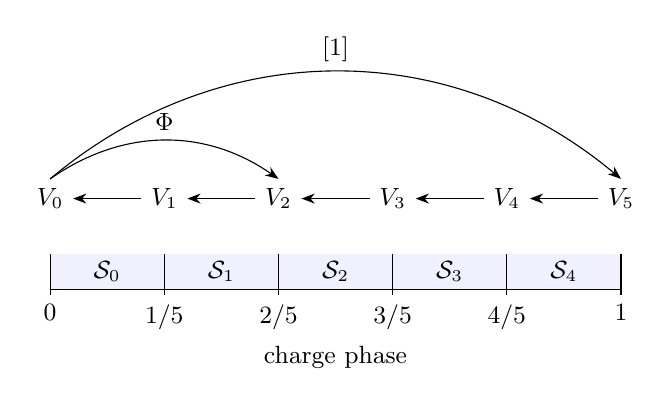
\begin{tikzpicture}[x=1.45cm,y=1cm,>=Stealth,
  every node/.style={font=\small}]
  \foreach \k in {0,...,5} {
    \node (v\k) at (\k,1.1) {$V_{\k}$};
  }
  \foreach \k in {0,...,4} {
    \pgfmathtruncatemacro{\next}{\k+1}
    \draw[->] (v\next.west) -- (v\k.east);
  }
  \draw[->] (v0.north) to[bend left=35]
    node[above] {$\Phi$} (v2.north);
  \draw[->] (v0.north) to[bend left=40]
    node[above] {$[1]$} (v5.north);
  \foreach \k in {0,...,4} {
    \fill[blue!6] (\k,-0.05) rectangle (\k+1,0.4);
    \node at (\k+0.5,0.175) {$\mathcal S_{\k}$};
  }
  \draw (0,-0.05) -- (5,-0.05);
  \foreach \k in {0,...,5} {
    \draw (\k,0.4) -- (\k,-0.12);
  }
  \node[below] at (0,-0.12) {$0$};
  \foreach \k in {1,...,4} {
    \node[below] at (\k,-0.12) {$\k/5$};
  }
  \node[below] at (5,-0.12) {$1$};
  \node[below] at (2.5,-0.65) {charge phase};
\end{tikzpicture}
\caption{The fifth-phase grid. Inclusion arrows point toward the larger
aisle. The autoequivalence $\Phi$ advances two indices, and the shift $[1]$
advances five. A nonzero object of $\mathcal S_k$ has charge phase in the
closed interval $[k/5,(k+1)/5]$, by Proposition~\ref{prop:block-support}.
At a shared endpoint, generators from both adjacent blocks enter the
definition of the slicing. The diagram shows the unperturbed grid;
Proposition~\ref{prop:fine-grid} gives the independent-parameter nesting.}
\label{fig:fifth-phase-grid}
\end{figure}


\subsection{Full numerical support on the blocks}

We first locate a block's charge using its two adjacent unperturbed hearts.
To bound its numerical class, we then place the same object in every perturbed
heart at the preceding grid position. This second step retains the two
independent inequalities that control rank and first Chern character.

\begin{proposition}\label{prop:block-support}
For the fixed Euclidean norm on $\Knum(X)_\R$, there is a constant $C>0$
such that, for every $k\in\Z$ and every nonzero $E\in\mathcal S_k$,
\begin{equation}\label{eq:block-support}
 \begin{gathered}
 Z(E)\in\{t e^{i\pi\varphi}:t>0,\ k/5\le\varphi\le(k+1)/5\},\\
 \norm{[E]}\le C|Z(E)|.
 \end{gathered}
\end{equation}
\end{proposition}

\begin{proof}
For $k=2m+5j$, the functor $\Phi^{-m}[-j]$ takes $\mathcal H_k$ to
$\mathcal A_0$ and multiplies its charge by $e^{-i\pi k/5}$.  Positivity
therefore gives $\Im(e^{-i\pi k/5}Z(E))\ge0$ on $\mathcal H_k$.
An object $E\in\mathcal S_k$ belongs both to $\mathcal H_k$ and to
\[
 \mathcal H_{k+1}[-1]
   =V_{k-4}\cap V_{k+1}^\perp.
\]
The two tests are consequently
\[
 \Im(e^{-i\pi k/5}Z(E))\ge0,\qquad
 \Im(e^{-i\pi(k+1)/5}Z(E))\le0.
\]
Their intersection is the closed sector in \eqref{eq:block-support},
together with the origin.

Choose $\varepsilon>0$ such that the closed square
$[-\varepsilon,\varepsilon]^2$ is contained in $\Omega_1$.
For every $\eta$ in this square, independent-parameter nesting gives
\[
 V_k\subset V_{k-1}^\eta,
 \qquad V_{k-1}^\eta[1]=V_{k+4}^\eta\subset V_{k+1}.
\]
Thus $E$ belongs to the heart of $V_{k-1}^\eta$ for every such $\eta$:
the second inclusion supplies exactly its required right orthogonality.
Write $k-1=2m+5j$, and set $w=[\Phi^{-m}E[-j]]$.  This is the class of an
actual object of $\mathcal A_\eta$ for every parameter under consideration,
including the shift in this formula.  Hence
\[
 N_0(w)+\eta_1c(w)+\eta_0r(w)\ge0
 \quad\text{for all }|\eta_0|,|\eta_1|\le\varepsilon.
\]
Choosing the two signs independently proves
\begin{equation}\label{eq:perturbed-support}
 \varepsilon\bigl(|r(w)|+|c(w)|\bigr)
 \le N_0(w)=\frac{\Im Z(w)}{5t_0}
 \le\frac{|Z(E)|}{5t_0}.
\end{equation}
The invertible real coordinate map
$w\mapsto(r(w),c(w),\Re Z(w),\Im Z(w))$, established in
\eqref{eq:numerical-norm-control}, now bounds $\norm{w}$ by a constant
times $|Z(E)|$.  Explicitly,
$d(w)=\Im Z(w)/(5t_0)-c(w)/2-ur(w)$, and then the real part of
\eqref{eq:central-charge} recovers $e(w)$.

We can choose $m\in\{0,1,2,3,4\}$ according to $k-1$ modulo five.
There are therefore only five norm-conversion operators $\Phi_*^m$;
the arbitrary shift $j$ only changes the sign of a numerical class.
Taking the maximum of their operator norms gives one $C$ for every $k$.
If $Z(E)=0$, the estimate gives $w=0$.  The object
$\Phi^{-m}E[-j]$ belongs to $\mathcal A_0$, so
Lemma~\ref{lem:second-tilt} forces $\Phi^{-m}E[-j]=0$ and hence $E=0$.
This excludes the origin for a nonzero block object and completes the proof.
\end{proof}

\subsection{Finite refinement inside a block}

The support estimate is now in place. We use it with the discreteness of the
full numerical lattice to obtain maximal phases and a bound on the length of
refinement; no discreteness of the charge image is needed.

Fix $k$, and put $a=k/5$, $b=(k+1)/5$.
Each nonzero $E\in\mathcal S_k$ has a unique phase
$\varphi_k(E)\in[a,b]$ with $Z(E)=|Z(E)|e^{i\pi\varphi_k(E)}$.
A subobject $F\subset E$ in $\mathcal H_k$ is called \emph{saturated in
the block} if $E/F\in\mathcal S_k$.  Its source already belongs to
$\mathcal S_k$ by Lemma~\ref{lem:block-filtrations}.  We call $E$
\emph{block-semistable} if
\[
 \varphi_k(F)\le\varphi_k(E)
 \quad\text{for every nonzero subobject saturated in the block.}
\]
The whole object is allowed as such a subobject.

\begin{lemma}[Finite block refinement]\label{lem:block-hn}
Every nonzero object of $\mathcal S_k$ has a finite filtration by short
exact sequences in $\mathcal H_k$, with all intermediate quotients in
$\mathcal S_k$, whose nonzero factors are block-semistable with strictly
decreasing phases.
\end{lemma}

\begin{proof}
Let $\ell>0$ be a lower bound for the norms of nonzero elements of the
full numerical lattice, supplied by Lemma~\ref{lem:numerical}, and define
\[
 q_k(z)=\Re\bigl(e^{-i\pi(a+b)/2}z\bigr),\qquad
 d_* =\frac{\ell\cos(\pi/10)}{C}>0.
\]
For every nonzero block object, Proposition~\ref{prop:block-support}
implies
\begin{equation}\label{eq:block-mass}
 q_k(Z(E))\ge\cos(\pi/10)|Z(E)|\ge d_*.
\end{equation}
This projection is additive in short exact sequences.  Hence every
filtration of a fixed $E$ with nonzero block factors has length at most
$q_k(Z(E))/d_*$.

If $F\subset E$ is saturated in the block, then both $F$ and $E/F$ are
block objects.  Their projections are nonnegative, so
\[
 \norm{[F]}\le C|Z(F)|
 \le \frac{C}{\cos(\pi/10)}q_k(Z(F))
 \le \frac{C}{\cos(\pi/10)}q_k(Z(E)).
\]
Only finitely many lattice classes, and therefore only finitely many
charges and phases, can occur for such $F$.  Choose a nonzero saturated
subobject $F\subset E$ of maximal phase, and among those of maximal
$|Z(F)|$.  These maxima concern finite sets of numerical values; no
finiteness of the set of subobjects is needed.

This $F$ is block-semistable.  Indeed, a saturated subobject of $F$ is
saturated in $E$, since the resulting quotient of $E$ is an extension of
two objects of $\mathcal S_k$.  If $G\subset E/F$ is a nonzero saturated
subobject, its preimage $\widetilde G\subset E$ is also saturated and is
an extension of $G$ by $F$.  Charges in a sector of width less than $\pi$
have the elementary strict see-saw property: the argument of their sum
is strictly between their arguments when those arguments differ, and
their magnitudes add when they agree.  Thus
$\varphi_k(G)>\varphi_k(F)$ contradicts maximal phase of $F$ by using
$\widetilde G$; equality contradicts maximal magnitude.  Every such $G$
therefore has phase strictly less than $\varphi_k(F)$.

Apply the same selection to the nonzero quotient $E/F$, if there is one,
and continue.  Preimages give a filtration in the original heart with all
factors and intermediate quotients in the block.  The phases strictly
decrease by the preceding argument, and \eqref{eq:block-mass} bounds the
number of nonzero factors, so the process terminates.
\end{proof}

\begin{lemma}[The unsaturated test and Hom vanishing]
\label{lem:block-hom}
If $E\in\mathcal S_k$ is block-semistable, then every nonzero subobject
$G\subset E$ in $\mathcal H_k$ satisfies
$\varphi_k(G)\le\varphi_k(E)$, without a saturation assumption.
Consequently, for block-semistable $E,F\in\mathcal S_k$,
\[
 \varphi_k(E)>\varphi_k(F)\quad\Longrightarrow\quad\Hom(E,F)=0.
\]
\end{lemma}

\begin{proof}
Suppose $G\subset E$ violates the stated inequality.  Decompose $E/G$
by \eqref{eq:block-torsion-pair} and take the preimage of its torsion
part:
\[
 0\longrightarrow T\longrightarrow E/G\longrightarrow F'\longrightarrow0,
 \qquad
 0\longrightarrow G\longrightarrow\overline G\longrightarrow T
      \longrightarrow0,
 \quad T\in\mathcal T_k,\ F'\in\mathcal S_k.
\]
The object $\overline G\subset E$ lies in $\mathcal S_k$ by subobject
closure, and is saturated because $E/\overline G=F'$.
The four-block filtration of $T$ has charge rays with phases in
$[b,a+1]$.  If $g=\varphi_k(G)$, then
\[
 a<g\le b,
 \qquad 0\le\psi-g\le a+1-g<1
 \quad\text{for every such phase }\psi.
\]
Thus $Z(G)$ and every added ray lie in the sector with phase interval
$[g,a+1]$ of width strictly less than one.  Their sum is nonzero and has
phase in that same interval.  Since $\overline G\in\mathcal S_k$, its
phase in $[a,b]$ must therefore be at least $g$.  In particular,
$\varphi_k(\overline G)>\varphi_k(E)$, a contradiction.
The strict inequality $g>a$, supplied by the alleged destabilization,
is what excludes an antipodal endpoint in this argument.  If $T=0$, the
contradiction already comes from $G$ itself being saturated.

For a nonzero map $E\to F$, take its image $I$ in $\mathcal H_k$.
Since $I\subset F$, we have $I\in\mathcal S_k$.  The kernel in $E$ is
therefore saturated.  If that kernel is zero, $\varphi_k(I)=\varphi_k(E)$;
otherwise semistability and the see-saw property give
$\varphi_k(I)\ge\varphi_k(E)$.  The unsaturated test applied to
$I\subset F$ gives $\varphi_k(I)\le\varphi_k(F)$.  These inequalities
exclude a nonzero map when the source phase is strictly larger.
\end{proof}

\subsection{The slicing and its phase cuts}

For $\varphi\in\R$, let $\mathcal P(\varphi)$ be the extension closure
of all block-semistable objects whose assigned phase equals $\varphi$.
There is one possible block unless $5\varphi\in\Z$, in which case the
two adjacent blocks are both included in this definition.

\begin{proposition}\label{prop:slicing}
The categories $\mathcal P(\varphi)$ form a slicing of $\D$ with finite
Harder--Narasimhan filtrations.  They satisfy
\begin{equation}\label{eq:slicing-covariance}
 \mathcal P(\varphi+1)=\mathcal P(\varphi)[1],\qquad
 \Phi\mathcal P(\varphi)=\mathcal P(\varphi+2/5)
 \quad(\varphi\in\R),
\end{equation}
and every nonzero $E\in\mathcal P(\varphi)$ satisfies
\begin{equation}\label{eq:semistable-support}
 Z(E)\in\R_{>0}e^{i\pi\varphi},\qquad
 \norm{[E]}\le C|Z(E)|.
\end{equation}
\end{proposition}

\begin{proof}
First consider the generators.  If two are in different blocks and the
source has strictly larger phase, its block index is larger: for $j<k$
one has $(j+1)/5\le k/5$.  Thus their Hom group vanishes by
Lemma~\ref{lem:block-filtrations}.  The case of a common block is
Lemma~\ref{lem:block-hom}.  Induction along extensions in each variable
now gives
\[
 \Hom(\mathcal P(\varphi),\mathcal P(\psi))=0
 \qquad(\varphi>\psi).
\]
The categories are additive, since finite direct sums are split
extensions.  The charge of an extension of phase-$\varphi$ generators
is a sum of positive multiples of $e^{i\pi\varphi}$ and hence is again
positive on that ray.  Likewise the triangle inequality gives
\[
 \norm{[E]}\le\sum_j\norm{[E_j]}
 \le C\sum_j|Z(E_j)|=C|Z(E)|
\]
for any such extension filtration.  This proves
\eqref{eq:semistable-support}.

Refine the decreasing block filtration of any object by
Lemma~\ref{lem:block-hn}, splicing the resulting triangles by the
octahedral axiom.  The phases are weakly decreasing globally and strictly
decreasing inside each block.  Adjacent equal phases can only occur at a
shared endpoint; merging each run of equal-phase factors into its
extension gives a finite filtration with strictly decreasing phases and
factors in the corresponding $\mathcal P(\varphi)$.  This also explains
why both blocks at a shared endpoint must enter the same phase category.

By \eqref{eq:fifths-nesting}, the functors $[1]$ and $\Phi$ take
$(\mathcal H_k,\mathcal S_k)$ to
$(\mathcal H_{k+5},\mathcal S_{k+5})$ and
$(\mathcal H_{k+2},\mathcal S_{k+2})$, respectively.  These equivalences
take exact sequences in the hearts to exact sequences, preserve the
condition of being saturated in a block, and change the assigned phase
by $1$ and $2/5$.  They therefore preserve block-semistability with these
phase increments.  Applying them and their inverses to the extension
closures proves both equalities in \eqref{eq:slicing-covariance}.
The phase-cut argument that follows proves closure under direct
summands without presupposing a slicing heart.
\end{proof}

For any interval $I\subset\R$, write $\mathcal P(I)$ for the extension
closure of the $\mathcal P(\varphi)$ with $\varphi\in I$.

\begin{lemma}[Direct construction of the phase cuts]\label{lem:phase-cuts}
For every real $c$, both pairs
\begin{equation}\label{eq:phase-cuts}
 \bigl(\mathcal P((c,\infty)),\mathcal P((-\infty,c])\bigr),
 \qquad
 \bigl(\mathcal P([c,\infty)),\mathcal P((-\infty,c))\bigr)
\end{equation}
are an aisle and its right orthogonal for a bounded t-structure.
Their hearts are respectively
$\mathcal P((c,c+1])$ and $\mathcal P([c,c+1))$.
Every interval category is the intersection of its lower and upper cut
categories, with the indicated endpoint conventions.  In particular,
these categories, including each $\mathcal P(\varphi)$, are closed under
direct summands.
\end{lemma}

\begin{proof}
Denote either pair in \eqref{eq:phase-cuts} by $(\mathcal U,\mathcal L)$.
Strict phase separation gives $\Hom(\mathcal U,\mathcal L)=0$ by
extension induction.  Equation~\eqref{eq:slicing-covariance} gives
$\mathcal U[1]\subset\mathcal U$ and
$\mathcal L[-1]\subset\mathcal L$.  Cutting the finite decreasing
filtration at $c$ and splicing triangles gives, for every $E$, a triangle
\begin{equation}\label{eq:phase-truncation}
 U_E\longrightarrow E\longrightarrow L_E\longrightarrow U_E[1],
 \qquad U_E\in\mathcal U,\ L_E\in\mathcal L.
\end{equation}
All factors of phase exactly $c$ are assigned to the same side, according
to the selected convention.  These are the t-structure axioms in the
aisle/right-orthogonal convention, and we can verify the orthogonal
characterizations directly before using any summand closure.  If
$E\in{}^\perp\mathcal L$, applying $\Hom(-,L_E)$ to
\eqref{eq:phase-truncation} shows that $\Hom(L_E,L_E)=0$, since its
neighboring terms $\Hom(U_E[1],L_E)$ and $\Hom(E,L_E)$ vanish.
Thus $L_E=0$ and $E\in\mathcal U$.  Similarly, if
$E\in\mathcal U^\perp$, apply $\Hom(U_E,-)$ and use
$\Hom(U_E,L_E[-1])=\Hom(U_E,E)=0$ to obtain $U_E=0$.
Hence
\[
 \mathcal U={}^\perp\mathcal L,\qquad
 \mathcal L=\mathcal U^\perp.
\]
They are consequently closed under direct summands, and
\eqref{eq:phase-truncation} is a genuine truncation triangle.  Finite
upper and lower bounds on the phases of each object's filtration, and
the shift law, prove boundedness.

We justify the interval description explicitly.  A nonempty decreasing
filtration with nonzero phase factors cannot have zero total object.
Indeed, the identity of its first factor maps nontrivially into the
total object: at each subsequent triangle this map remains nonzero
because $\Hom(F_1,F_j[-1])=0$.  Now group a chosen filtration of an
object at the two endpoints of an interval.  If the object lies in the
upper and lower cut categories, the preceding orthogonal
characterizations force the exterior truncation objects to be zero.
By the observation just made, their groups of factors are empty.  The
remaining factors lie in the interval.  The reverse inclusion follows
from extension closure.  This works with either choice at either
endpoint, as well as for rays and singletons.
Intersecting the aisle with the right orthogonal of its shift therefore
gives precisely the two displayed hearts.  Finally, intersections of
orthogonals are closed under summands, which proves the last assertion.
\end{proof}

\subsection{Quasi-abelian intervals and local finite length}

It remains to verify local finiteness. We first identify the exact sequences
in a short phase interval by realizing it inside a phase-cut heart. We then
use a positive projection of the charge to bound the length of every strict
filtration in that interval.

\begin{lemma}[The exact structure on a short phase interval]
\label{lem:interval-quasiabelian}
For every interval $I$ of width less than one, with any choices of open
or closed endpoints, $\mathcal P(I)$ is quasi-abelian.  Its strict exact
sequences are exactly the short exact sequences of a suitable bounded
heart whose three terms belong to $\mathcal P(I)$.
\end{lemma}

\begin{proof}
The empty interval gives the zero category.  Otherwise let $a\le b$
be its endpoints, with $b-a<1$.  If $a$ is excluded, use the heart
$\mathcal H=\mathcal P((a,a+1])$; if it is included, use
$\mathcal H=\mathcal P([a,a+1))$.  Inside this heart, the cut at $b$
gives a torsion pair $(\mathcal T,\mathcal F)$ with
$\mathcal F=\mathcal P(I)$.  Equality at $b$ is assigned to
$\mathcal F$ exactly when $b\in I$.  For example, for $I=(a,b)$ it is
\[
 \mathcal T=\mathcal P([b,a+1]),\qquad
 \mathcal F=\mathcal P((a,b))
 \quad\text{in }\mathcal P((a,a+1]).
\]
For $I=(a,b]$ the corresponding torsion class is
$\mathcal P((b,a+1])$.  The lower-closed variants use the other heart
above and the same upper-endpoint rule.  Hom orthogonality follows from
the phase inequality, and the cut triangles have all terms in
$\mathcal H$, so they give the required short exact decompositions.

We prove the quasi-abelian assertion directly for a torsion-free class
$\mathcal F$ in an abelian heart $\mathcal H$; this standard fact is also
recorded in \cite[Lemma~3.1]{Tattar2021}.
It is closed under subobjects and extensions.  For a morphism
$f:A\to B$ in $\mathcal F$, put
$K=\ker_{\mathcal H}f$, $J=\im_{\mathcal H}f$, and
$Q=\operatorname{coker}_{\mathcal H}f$.
The kernel in $\mathcal F$ is $K$, and the cokernel is
$Q/t(Q)$, where $t(Q)$ denotes the torsion part of $Q$.
Indeed, maps from $Q$ to an object of $\mathcal F$ annihilate $t(Q)$;
this proves the cokernel's universal property.  Both $K$ and $J$ lie in
$\mathcal F$.  Consequently the internal coimage of $f$ is $J$, whereas
its internal image is the preimage of $t(Q)$ under $B\to Q$.

Recall that a morphism is strict if its canonical coimage-to-image map
is an isomorphism.  The preceding formulas show that a strict
monomorphism in $\mathcal F$ is exactly a monomorphism in $\mathcal H$
whose cokernel belongs to $\mathcal F$.  A strict epimorphism in
$\mathcal F$ is exactly an epimorphism in $\mathcal H$ between its
objects: for an internal epimorphism the internal image is $B$, and
strictness says precisely that $J=B$.  This statement is about strict
epimorphisms, not all epimorphisms of the subcategory.

The pushout in $\mathcal H$ of a strict monomorphism $A\hookrightarrow B$
along $A\to A'$ fits into
\[
 0\longrightarrow A'\longrightarrow B'\longrightarrow B/A
     \longrightarrow0.
\]
Both outside terms are in $\mathcal F$, so $B'\in\mathcal F$ and the
new monomorphism is strict.  The pullback in $\mathcal H$ of a strict
epimorphism $A\twoheadrightarrow B$ along $B'\to B$ is a subobject of
$A\oplus B'$, hence lies in $\mathcal F$, and its projection to $B'$ is
an ambient epimorphism, hence strict.  These ambient universal
properties remain universal in the full subcategory $\mathcal F$.
Thus kernels and cokernels exist, pushouts preserve strict
monomorphisms, and pullbacks preserve strict epimorphisms.  This proves
quasi-abelianity and the stated description of strict exact sequences.
\end{proof}

\begin{proposition}[Local finiteness]\label{prop:local-finiteness}
Every phase interval of width less than one generates a finite-length
quasi-abelian category.  Hence the slicing in
Proposition~\ref{prop:slicing} is locally finite.
\end{proposition}

\begin{proof}
Let $I$ have endpoints $a\le b$ and width $w=b-a<1$, and put
\[
 q_I(z)=\Re\bigl(e^{-i\pi(a+b)/2}z\bigr),\qquad
 d_I=\frac{\ell}{C}\cos(\pi w/2)>0,
\]
where $\ell$ is the full-lattice norm lower bound used in
Lemma~\ref{lem:block-hn}.  A nonzero semistable $F$ of phase in $I$ has
nonzero numerical class, since its charge is nonzero.  Therefore
\eqref{eq:semistable-support} gives
\[
 q_I(Z(F))\ge\cos(\pi w/2)|Z(F)|\ge d_I.
\]
Every nonzero object of $\mathcal P(I)$ is a finite extension of nonzero
semistable objects with phases in $I$.  Additivity thus gives the same
lower bound $q_I(Z(E))\ge d_I$ for every such object.

By Lemma~\ref{lem:interval-quasiabelian}, a strict exact sequence in
$\mathcal P(I)$ is exact in its ambient heart, so the projection $q_I Z$
is additive on it.  Every nonzero successive quotient in a strict
filtration of a fixed $E\in\mathcal P(I)$ is again an object of
$\mathcal P(I)$ and consumes at least $d_I$ of this projection.
The number of such quotients is consequently at most
$q_I(Z(E))/d_I$.  This bounds both increasing and decreasing strict
subobject chains, and proves finite length in the quasi-abelian exact
structure.  The argument uses discreteness of the full numerical
lattice; it requires no discreteness of its image under $Z$.
\end{proof}

The charge is numerical and normalized on point sheaves by
Proposition~\ref{prop:central-charge}; its eigencharge identity combines
with \eqref{eq:slicing-covariance}.  Proposition~\ref{prop:slicing},
Lemma~\ref{lem:phase-cuts}, and Proposition~\ref{prop:local-finiteness}
give all slicing, Harder--Narasimhan, and local-finiteness requirements.
Finally \eqref{eq:semistable-support} is the support property on the
\emph{full} space $\Knum(X)_\R$.  This completes the proof of
Theorem~\ref{thm:main}.

\appendix
\section{A relative-kernel proof of periodicity}
\label{app:periodicity}

\begin{proof}[Proof of Lemma~\ref{lem:periodicity}]
Write $T_j=T_{\OO_X(j)}$ and $L=(-\otimes\OO_X(1))$.
We interpret the twist as the Fourier--Mukai transform whose kernel is
the cone of the evaluation map
\[
 \OO_X(-j)\boxtimes\OO_X(j)\longrightarrow\OO_\Delta.
\]
We take cones in the standard enhancement by complexes of perfect
kernels, so that the evaluation squares below induce maps of cones.
Their transforms give natural transformations of functors. Tensoring the evaluation
kernel gives $LT_jL^{-1}\simeq T_{j+1}$, and hence
\begin{equation}\label{eq:twist-product}
 \Phi^5\simeq T_0T_1T_2T_3T_4L^5.
\end{equation}
We will identify the kernel of $T_0T_1T_2T_3T_4$ with
$\OO_\Delta(-5)[2]$, where the twist is in the second factor.

Keep the first copy of $X$ as a source parameter. Set
\[
 f=1_X\times i\colon X\times X\longrightarrow X\times\mathbf P^4,
 \qquad
 p\colon X\times\mathbf P^4\longrightarrow X,
 \quad q\colon X\times X\longrightarrow X.
\]
Here $p$ and $q$ are the first projections.
The kernel convention is that $F\in\Db(\Coh(X\times Y))$ sends $E$ to
$R\pi_{Y*}(\pi_X^*E\otimes^{\mathbf L}F)$.
For such a kernel, let
\[
 a_j^Y(F)=R\pi_{X*}\bigl(F\otimes\pi_Y^*\OO_Y(-j)\bigr),
 \qquad
 \mathsf L_j^Y(F)=
 \operatorname{Cone}\bigl(a_j^Y(F)\boxtimes\OO_Y(j)\longrightarrow F\bigr).
\]
The arrow is the adjunction evaluation. Projection formula and proper
base change show that $\mathsf L_j^Y(F)$ represents postcomposition of
the transform of $F$ with the evaluation cone for $\OO_Y(j)$.
Indeed, on an input $E$ the first kernel in this cone gives
\[
 R\Gamma\bigl(X,E\otimes^{\mathbf L}a_j^Y(F)\bigr)\otimes\OO_Y(j)
 \simeq
 R\operatorname{Hom}\bigl(\OO_Y(j),\Phi_F(E)\bigr)\otimes\OO_Y(j).
\]
In particular the source coefficient here is $a_j^Y(F)$ itself.

These coefficient functors let us compare the evaluation cones on $X$ with
those on $\mathbf P^4$. We will show that the five projective-space
evaluations remove all coefficients and leave the zero kernel, while the
comparison preserves the cone of the divisor counit. Computing that cone
will give the required shift.

Start with
\[
 K_5=f_*\OO_\Delta,\qquad G_5=\OO_\Delta,\qquad
 u_5\colon Lf^*K_5\longrightarrow G_5
\]
given by the counit. For $j=4,3,\ldots,0$, form successively
\[
 K_j=\mathsf L_j^{\mathbf P^4}(K_{j+1}),
 \qquad
 G_j=\mathsf L_j^X(G_{j+1}).
\]
We construct compatible maps $u_j\colon Lf^*K_j\to G_j$ and show
that their cones are all isomorphic to $\operatorname{Cone}(u_5)$.

For any map $u\colon Lf^*K\to G$, the unit followed by $f_*u$ gives
$K\to f_*G$, hence comparison maps
\[
 \theta_l\colon a_l^{\mathbf P^4}(K)\longrightarrow a_l^X(G).
\]
For $(K_5,G_5,u_5)$ these are isomorphisms for every $l$: the composite
$f_*\OO_\Delta\to f_*Lf^*f_*\OO_\Delta\to f_*\OO_\Delta$
is the identity by the adjunction identity. Suppose that, before the
step indexed by $j$, the maps $\theta_l$ are isomorphisms for
$0\le l\le j$. The evaluation square
\[
\begin{array}{ccc}
 q^*a_j^{\mathbf P^4}(K_{j+1})\otimes\OO_X(j)
   &\longrightarrow& Lf^*K_{j+1}\\
 \big\downarrow\scriptstyle{\simeq}&&\big\downarrow\scriptstyle{u_{j+1}}\\
 q^*a_j^X(G_{j+1})\otimes\OO_X(j)
   &\longrightarrow& G_{j+1}
\end{array}
\]
commutes by adjunction. Taking its cones defines $u_j$; because its
left vertical arrow is an isomorphism, the cone of $u_j$ is isomorphic
to the cone of $u_{j+1}$.

For $l<j$, apply the coefficient functor $a_l$ to the two evaluation
triangles. The comparison on their first terms is
\[
 a_j^{\mathbf P^4}(K_{j+1})\otimes R\Gamma(\mathbf P^4,\OO(j-l))
 \longrightarrow
 a_j^X(G_{j+1})\otimes R\Gamma(X,\OO_X(j-l)).
\]
It is an isomorphism: $\theta_j$ is an isomorphism, and the divisor
sequence
\[
 0\longrightarrow\OO_{\mathbf P^4}(m-5)
 \longrightarrow\OO_{\mathbf P^4}(m)
 \longrightarrow i_*\OO_X(m)\longrightarrow0
\]
identifies the two cohomology complexes for $1\le m\le4$.
The comparison on the middle terms is also an isomorphism by induction,
so the remaining maps $\theta_l$ stay isomorphisms after the mutation.
This proves the induction and the constancy of the cone.

We next show that $K_0=0$. The step indexed by $j$ kills
$a_j^{\mathbf P^4}$, since
$R\Gamma(\mathbf P^4,\OO)=\C$. It preserves the already vanishing
coefficients with indices $k>j$, since
$R\Gamma(\mathbf P^4,\OO(j-k))=0$ for $1\le k-j\le4$.
Thus $a_j^{\mathbf P^4}(K_0)=0$ for $0\le j\le4$.
All these kernels are perfect, and proper base change implies that
every derived source fiber $F$ of $K_0$ satisfies
\[
 R\operatorname{Hom}_{\mathbf P^4}(\OO(j),F)=0
 \qquad(0\le j\le4).
\]
The exact Koszul complex of the five homogeneous coordinates propagates
these five consecutive vanishings to
$R\Gamma(\mathbf P^4,F(n))=0$ for every integer $n$.
For sufficiently large $n$, Serre vanishing and global generation,
applied to the finitely many cohomology sheaves of $F$, force all those
sheaves to vanish. Therefore every derived source fiber is zero, and
the derived Nakayama lemma gives $K_0=0$. It follows that
\[
 G_0\simeq\operatorname{Cone}(u_0)
       \simeq\operatorname{Cone}(u_5).
\]

Finally, $f$ is a Cartier divisor embedding with normal bundle
$\OO_X(5)$ in the target variable. Its two-term divisor resolution
computes
\[
 \mathcal H^{-1}(Lf^*f_*\OO_\Delta)=\OO_\Delta(-5),
 \qquad
 \mathcal H^0(Lf^*f_*\OO_\Delta)=\OO_\Delta,
\]
with no other cohomology sheaves. The counit $u_5$ induces the identity
in degree zero. Consequently its cone has the single cohomology sheaf
$\OO_\Delta(-5)$ in degree $-2$, and
\[
 G_0\simeq\OO_\Delta(-5)[2].
\]
Since $G_0$ is the composition kernel for $T_0T_1T_2T_3T_4$, this is
an isomorphism of kernels and therefore a natural functor isomorphism.
Equation~\eqref{eq:twist-product} now gives $\Phi^5\simeq[2]$.
The asserted inverse follows by composing this relation with $[-2]$.
\end{proof}

\bibliographystyle{plain}
\bibliography{references}
\end{document}
